\documentclass{standalone}
\usepackage{tikz}
\usetikzlibrary{patterns, positioning}

\begin{document}
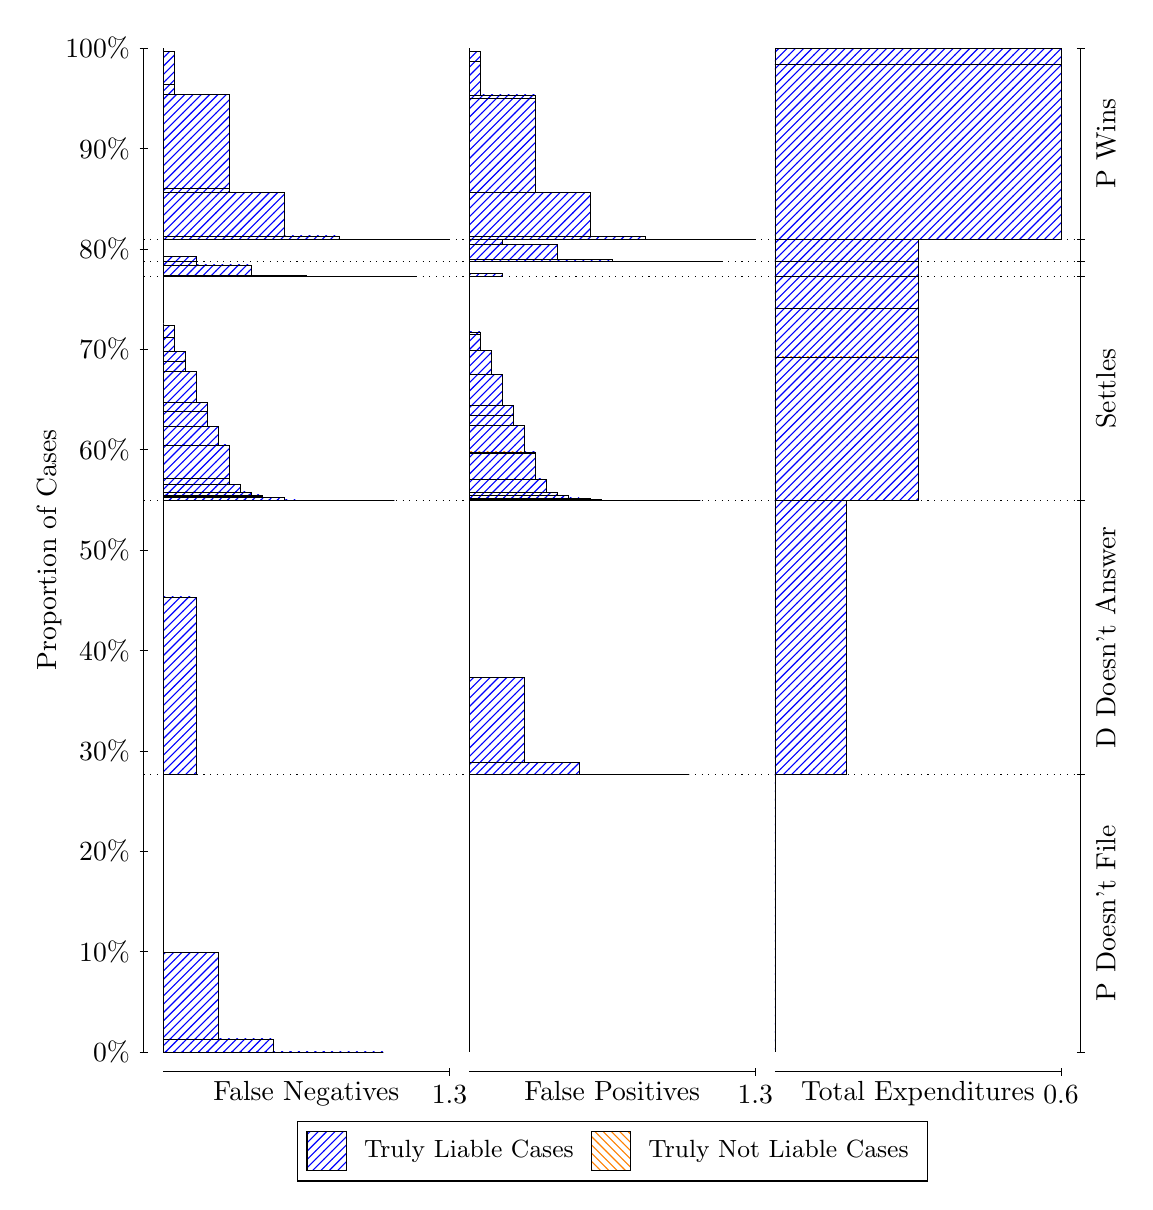
\begin{tikzpicture}
\draw[black, very thin] (1.5,1.75) -- (1.5,14.5);
\node[rotate=90, anchor=center] at (0.3, 8.125) {Proportion of Cases};
\draw[black, very thin] (1.45,1.75) -- (1.55,1.75);
\node[anchor=east] at (1.45, 1.75) {0\%};
\draw[black, very thin] (1.45,3.025) -- (1.55,3.025);
\node[anchor=east] at (1.45, 3.025) {10\%};
\draw[black, very thin] (1.45,4.3) -- (1.55,4.3);
\node[anchor=east] at (1.45, 4.3) {20\%};
\draw[black, very thin] (1.45,5.575) -- (1.55,5.575);
\node[anchor=east] at (1.45, 5.575) {30\%};
\draw[black, very thin] (1.45,6.85) -- (1.55,6.85);
\node[anchor=east] at (1.45, 6.85) {40\%};
\draw[black, very thin] (1.45,8.125) -- (1.55,8.125);
\node[anchor=east] at (1.45, 8.125) {50\%};
\draw[black, very thin] (1.45,9.4) -- (1.55,9.4);
\node[anchor=east] at (1.45, 9.4) {60\%};
\draw[black, very thin] (1.45,10.675) -- (1.55,10.675);
\node[anchor=east] at (1.45, 10.675) {70\%};
\draw[black, very thin] (1.45,11.95) -- (1.55,11.95);
\node[anchor=east] at (1.45, 11.95) {80\%};
\draw[black, very thin] (1.45,13.225) -- (1.55,13.225);
\node[anchor=east] at (1.45, 13.225) {90\%};
\draw[black, very thin] (1.45,14.5) -- (1.55,14.5);
\node[anchor=east] at (1.45, 14.5) {100\%};

\draw[black, very thin] (13.4,1.75) -- (13.4,14.5);
\draw[black, very thin] (13.35,1.75) -- (13.45,1.75);
\node[anchor=west] at (13.35, 1.75) {};
\draw[black, very thin] (13.35,5.2766) -- (13.45,5.2766);
\node[anchor=west] at (13.35, 5.2766) {};
\draw[black, very thin] (13.35,8.7586) -- (13.45,8.7586);
\node[anchor=west] at (13.35, 8.7586) {};
\draw[black, very thin] (13.35,11.596) -- (13.45,11.596);
\node[anchor=west] at (13.35, 11.596) {};
\draw[black, very thin] (13.35,11.791) -- (13.45,11.791);
\node[anchor=west] at (13.35, 11.791) {};
\draw[black, very thin] (13.35,12.071) -- (13.45,12.071);
\node[anchor=west] at (13.35, 12.071) {};
\draw[black, very thin] (13.35,14.5) -- (13.45,14.5);
\node[anchor=west] at (13.35, 14.5) {};

\draw[black, very thin, pattern color=blue, pattern=north east lines] (1.75,1.75) rectangle (4.5449,1.75);
\draw[black, very thin, pattern color=blue, pattern=north east lines] (1.75,1.75) rectangle (3.8462,1.7514);
\draw[black, very thin, pattern color=blue, pattern=north east lines] (1.75,1.7514) rectangle (3.1474,1.9157);
\draw[black, very thin, pattern color=blue, pattern=north east lines] (1.75,1.9157) rectangle (2.4487,3.0163);
\draw[black, very thin, pattern color=orange, pattern=north west lines] (1.75,3.0163) rectangle (1.75,3.0163);
\draw[black, very thin, pattern color=blue, pattern=north east lines] (1.75,3.0163) rectangle (1.75,5.2766);
\draw[black, very thin, pattern color=blue, pattern=north east lines] (1.75,5.2766) rectangle (2.1692,7.5308);
\draw[black, very thin, pattern color=orange, pattern=north west lines] (1.75,7.5308) rectangle (1.75,7.5308);
\draw[black, very thin, pattern color=blue, pattern=north east lines] (1.75,7.5308) rectangle (1.75,8.7586);
\draw[black, very thin, pattern color=blue, pattern=north east lines] (1.75,8.7586) rectangle (4.6846,8.7586);
\draw[black, very thin, pattern color=blue, pattern=north east lines] (1.75,8.7586) rectangle (4.4051,8.7586);
\draw[black, very thin, pattern color=blue, pattern=north east lines] (1.75,8.7586) rectangle (4.1256,8.7586);
\draw[black, very thin, pattern color=blue, pattern=north east lines] (1.75,8.7586) rectangle (3.9859,8.7586);
\draw[black, very thin, pattern color=blue, pattern=north east lines] (1.75,8.7586) rectangle (3.8462,8.7586);
\draw[black, very thin, pattern color=blue, pattern=north east lines] (1.75,8.7586) rectangle (3.7064,8.7587);
\draw[black, very thin, pattern color=blue, pattern=north east lines] (1.75,8.7587) rectangle (3.5667,8.7589);
\draw[black, very thin, pattern color=blue, pattern=north east lines] (1.75,8.7589) rectangle (3.4269,8.7609);
\draw[black, very thin, pattern color=blue, pattern=north east lines] (1.75,8.7609) rectangle (3.2872,8.7898);
\draw[black, very thin, pattern color=blue, pattern=north east lines] (1.75,8.7898) rectangle (3.1474,8.794);
\draw[black, very thin, pattern color=blue, pattern=north east lines] (1.75,8.794) rectangle (3.0077,8.8024);
\draw[black, very thin, pattern color=blue, pattern=north east lines] (1.75,8.8024) rectangle (3.0077,8.8253);
\draw[black, very thin, pattern color=blue, pattern=north east lines] (1.75,8.8253) rectangle (2.8679,8.8643);
\draw[black, very thin, pattern color=blue, pattern=north east lines] (1.75,8.8643) rectangle (2.7282,8.9623);
\draw[black, very thin, pattern color=blue, pattern=north east lines] (1.75,8.9623) rectangle (2.5885,9.0303);
\draw[black, very thin, pattern color=blue, pattern=north east lines] (1.75,9.0303) rectangle (2.5885,9.4602);
\draw[black, very thin, pattern color=blue, pattern=north east lines] (1.75,9.4602) rectangle (2.4487,9.6955);
\draw[black, very thin, pattern color=blue, pattern=north east lines] (1.75,9.6955) rectangle (2.309,9.8881);
\draw[black, very thin, pattern color=blue, pattern=north east lines] (1.75,9.8881) rectangle (2.309,9.9964);
\draw[black, very thin, pattern color=blue, pattern=north east lines] (1.75,9.9964) rectangle (2.1692,10.395);
\draw[black, very thin, pattern color=blue, pattern=north east lines] (1.75,10.395) rectangle (2.0295,10.516);
\draw[black, very thin, pattern color=blue, pattern=north east lines] (1.75,10.516) rectangle (2.0295,10.645);
\draw[black, very thin, pattern color=blue, pattern=north east lines] (1.75,10.645) rectangle (1.8897,10.821);
\draw[black, very thin, pattern color=blue, pattern=north east lines] (1.75,10.821) rectangle (1.8897,10.982);
\draw[black, very thin, pattern color=blue, pattern=north east lines] (1.75,10.982) rectangle (1.75,11.001);
\draw[black, very thin, pattern color=orange, pattern=north west lines] (1.75,11.001) rectangle (1.75,11.001);
\draw[black, very thin, pattern color=blue, pattern=north east lines] (1.75,11.001) rectangle (1.75,11.596);
\draw[black, very thin, pattern color=blue, pattern=north east lines] (1.75,11.596) rectangle (4.9641,11.596);
\draw[black, very thin, pattern color=blue, pattern=north east lines] (1.75,11.596) rectangle (4.2654,11.596);
\draw[black, very thin, pattern color=blue, pattern=north east lines] (1.75,11.596) rectangle (3.5667,11.612);
\draw[black, very thin, pattern color=blue, pattern=north east lines] (1.75,11.612) rectangle (2.8679,11.747);
\draw[black, very thin, pattern color=blue, pattern=north east lines] (1.75,11.747) rectangle (2.1692,11.791);
\draw[black, very thin, pattern color=orange, pattern=north west lines] (1.75,11.791) rectangle (1.75,11.791);
\draw[black, very thin, pattern color=blue, pattern=north east lines] (1.75,11.791) rectangle (2.1692,11.857);
\draw[black, very thin, pattern color=orange, pattern=north west lines] (1.75,11.857) rectangle (1.75,11.857);
\draw[black, very thin, pattern color=blue, pattern=north east lines] (1.75,11.857) rectangle (1.75,12.071);
\draw[black, very thin, pattern color=blue, pattern=north east lines] (1.75,12.071) rectangle (5.3833,12.071);
\draw[black, very thin, pattern color=blue, pattern=north east lines] (1.75,12.071) rectangle (4.6846,12.072);
\draw[black, very thin, pattern color=blue, pattern=north east lines] (1.75,12.072) rectangle (3.9859,12.113);
\draw[black, very thin, pattern color=blue, pattern=north east lines] (1.75,12.113) rectangle (3.2872,12.667);
\draw[black, very thin, pattern color=blue, pattern=north east lines] (1.75,12.667) rectangle (2.5885,12.725);
\draw[black, very thin, pattern color=blue, pattern=north east lines] (1.75,12.725) rectangle (2.5885,13.909);
\draw[black, very thin, pattern color=blue, pattern=north east lines] (1.75,13.909) rectangle (1.8897,14.039);
\draw[black, very thin, pattern color=blue, pattern=north east lines] (1.75,14.039) rectangle (1.8897,14.459);
\draw[black, very thin, pattern color=orange, pattern=north west lines] (1.75,14.459) rectangle (1.75,14.459);
\draw[black, very thin, pattern color=blue, pattern=north east lines] (1.75,14.459) rectangle (1.75,14.5);
\draw[black, very thin, pattern color=orange, pattern=north west lines] (5.6333,1.75) rectangle (5.6333,1.75);
\draw[black, very thin, pattern color=blue, pattern=north east lines] (5.6333,1.75) rectangle (5.6333,5.2766);
\draw[black, very thin, pattern color=orange, pattern=north west lines] (5.6333,5.2766) rectangle (8.4282,5.2766);
\draw[black, very thin, pattern color=blue, pattern=north east lines] (5.6333,5.2766) rectangle (8.4282,5.2766);
\draw[black, very thin, pattern color=blue, pattern=north east lines] (5.6333,5.2766) rectangle (7.7295,5.2773);
\draw[black, very thin, pattern color=blue, pattern=north east lines] (5.6333,5.2773) rectangle (7.0308,5.4263);
\draw[black, very thin, pattern color=blue, pattern=north east lines] (5.6333,5.4263) rectangle (6.3321,6.5043);
\draw[black, very thin, pattern color=blue, pattern=north east lines] (5.6333,6.5043) rectangle (5.6333,8.7586);
\draw[black, very thin, pattern color=orange, pattern=north west lines] (5.6333,8.7586) rectangle (8.5679,8.7586);
\draw[black, very thin, pattern color=blue, pattern=north east lines] (5.6333,8.7586) rectangle (8.5679,8.7586);
\draw[black, very thin, pattern color=orange, pattern=north west lines] (5.6333,8.7586) rectangle (8.2885,8.7586);
\draw[black, very thin, pattern color=blue, pattern=north east lines] (5.6333,8.7586) rectangle (8.2885,8.7586);
\draw[black, very thin, pattern color=orange, pattern=north west lines] (5.6333,8.7586) rectangle (8.009,8.7586);
\draw[black, very thin, pattern color=blue, pattern=north east lines] (5.6333,8.7586) rectangle (8.009,8.7586);
\draw[black, very thin, pattern color=blue, pattern=north east lines] (5.6333,8.7586) rectangle (7.8692,8.7586);
\draw[black, very thin, pattern color=orange, pattern=north west lines] (5.6333,8.7586) rectangle (7.7295,8.7586);
\draw[black, very thin, pattern color=blue, pattern=north east lines] (5.6333,8.7586) rectangle (7.7295,8.7586);
\draw[black, very thin, pattern color=blue, pattern=north east lines] (5.6333,8.7586) rectangle (7.5897,8.7587);
\draw[black, very thin, pattern color=orange, pattern=north west lines] (5.6333,8.7587) rectangle (7.45,8.7587);
\draw[black, very thin, pattern color=blue, pattern=north east lines] (5.6333,8.7587) rectangle (7.45,8.7588);
\draw[black, very thin, pattern color=blue, pattern=north east lines] (5.6333,8.7588) rectangle (7.3103,8.7641);
\draw[black, very thin, pattern color=orange, pattern=north west lines] (5.6333,8.7641) rectangle (7.1705,8.7641);
\draw[black, very thin, pattern color=blue, pattern=north east lines] (5.6333,8.7641) rectangle (7.1705,8.78);
\draw[black, very thin, pattern color=orange, pattern=north west lines] (5.6333,8.78) rectangle (7.1705,8.78);
\draw[black, very thin, pattern color=blue, pattern=north east lines] (5.6333,8.78) rectangle (7.1705,8.7801);
\draw[black, very thin, pattern color=blue, pattern=north east lines] (5.6333,8.7801) rectangle (7.0308,8.7881);
\draw[black, very thin, pattern color=blue, pattern=north east lines] (5.6333,8.7881) rectangle (6.891,8.8187);
\draw[black, very thin, pattern color=orange, pattern=north west lines] (5.6333,8.8187) rectangle (6.891,8.8187);
\draw[black, very thin, pattern color=blue, pattern=north east lines] (5.6333,8.8187) rectangle (6.891,8.8229);
\draw[black, very thin, pattern color=blue, pattern=north east lines] (5.6333,8.8229) rectangle (6.7513,8.8586);
\draw[black, very thin, pattern color=orange, pattern=north west lines] (5.6333,8.8586) rectangle (6.6115,8.8586);
\draw[black, very thin, pattern color=blue, pattern=north east lines] (5.6333,8.8586) rectangle (6.6115,9.0269);
\draw[black, very thin, pattern color=blue, pattern=north east lines] (5.6333,9.0269) rectangle (6.4718,9.3532);
\draw[black, very thin, pattern color=blue, pattern=north east lines] (5.6333,9.3532) rectangle (6.4718,9.3724);
\draw[black, very thin, pattern color=orange, pattern=north west lines] (5.6333,9.3724) rectangle (6.3321,9.3724);
\draw[black, very thin, pattern color=blue, pattern=north east lines] (5.6333,9.3724) rectangle (6.3321,9.7094);
\draw[black, very thin, pattern color=blue, pattern=north east lines] (5.6333,9.7094) rectangle (6.1923,9.8387);
\draw[black, very thin, pattern color=blue, pattern=north east lines] (5.6333,9.8387) rectangle (6.1923,9.959);
\draw[black, very thin, pattern color=blue, pattern=north east lines] (5.6333,9.959) rectangle (6.0526,10.358);
\draw[black, very thin, pattern color=blue, pattern=north east lines] (5.6333,10.358) rectangle (5.9128,10.659);
\draw[black, very thin, pattern color=blue, pattern=north east lines] (5.6333,10.659) rectangle (5.7731,10.87);
\draw[black, very thin, pattern color=blue, pattern=north east lines] (5.6333,10.87) rectangle (5.7731,10.894);
\draw[black, very thin, pattern color=blue, pattern=north east lines] (5.6333,10.894) rectangle (5.6333,11.596);
\draw[black, very thin, pattern color=orange, pattern=north west lines] (5.6333,11.596) rectangle (6.0526,11.596);
\draw[black, very thin, pattern color=blue, pattern=north east lines] (5.6333,11.596) rectangle (6.0526,11.64);
\draw[black, very thin, pattern color=blue, pattern=north east lines] (5.6333,11.64) rectangle (5.6333,11.791);
\draw[black, very thin, pattern color=orange, pattern=north west lines] (5.6333,11.791) rectangle (8.8474,11.791);
\draw[black, very thin, pattern color=blue, pattern=north east lines] (5.6333,11.791) rectangle (8.8474,11.791);
\draw[black, very thin, pattern color=blue, pattern=north east lines] (5.6333,11.791) rectangle (8.1487,11.791);
\draw[black, very thin, pattern color=blue, pattern=north east lines] (5.6333,11.791) rectangle (7.45,11.814);
\draw[black, very thin, pattern color=blue, pattern=north east lines] (5.6333,11.814) rectangle (6.7513,12.005);
\draw[black, very thin, pattern color=blue, pattern=north east lines] (5.6333,12.005) rectangle (6.0526,12.071);
\draw[black, very thin, pattern color=orange, pattern=north west lines] (5.6333,12.071) rectangle (9.2667,12.071);
\draw[black, very thin, pattern color=blue, pattern=north east lines] (5.6333,12.071) rectangle (9.2667,12.071);
\draw[black, very thin, pattern color=orange, pattern=north west lines] (5.6333,12.071) rectangle (8.5679,12.071);
\draw[black, very thin, pattern color=blue, pattern=north east lines] (5.6333,12.071) rectangle (8.5679,12.072);
\draw[black, very thin, pattern color=orange, pattern=north west lines] (5.6333,12.072) rectangle (7.8692,12.072);
\draw[black, very thin, pattern color=blue, pattern=north east lines] (5.6333,12.072) rectangle (7.8692,12.112);
\draw[black, very thin, pattern color=orange, pattern=north west lines] (5.6333,12.112) rectangle (7.1705,12.112);
\draw[black, very thin, pattern color=blue, pattern=north east lines] (5.6333,12.112) rectangle (7.1705,12.662);
\draw[black, very thin, pattern color=blue, pattern=north east lines] (5.6333,12.662) rectangle (6.4718,13.856);
\draw[black, very thin, pattern color=orange, pattern=north west lines] (5.6333,13.856) rectangle (6.4718,13.856);
\draw[black, very thin, pattern color=blue, pattern=north east lines] (5.6333,13.856) rectangle (6.4718,13.904);
\draw[black, very thin, pattern color=blue, pattern=north east lines] (5.6333,13.904) rectangle (5.7731,14.329);
\draw[black, very thin, pattern color=blue, pattern=north east lines] (5.6333,14.329) rectangle (5.7731,14.459);
\draw[black, very thin, pattern color=blue, pattern=north east lines] (5.6333,14.459) rectangle (5.6333,14.5);
\draw[black, very thin, pattern color=orange, pattern=north west lines] (9.5167,1.75) rectangle (9.5167,1.75);
\draw[black, very thin, pattern color=blue, pattern=north east lines] (9.5167,1.75) rectangle (9.5167,5.2766);
\draw[black, very thin, pattern color=orange, pattern=north west lines] (9.5167,5.2766) rectangle (10.425,5.2766);
\draw[black, very thin, pattern color=blue, pattern=north east lines] (9.5167,5.2766) rectangle (10.425,8.7586);
\draw[black, very thin, pattern color=orange, pattern=north west lines] (9.5167,8.7586) rectangle (11.333,8.7586);
\draw[black, very thin, pattern color=blue, pattern=north east lines] (9.5167,8.7586) rectangle (11.333,10.578);
\draw[black, very thin, pattern color=orange, pattern=north west lines] (9.5167,10.578) rectangle (11.333,10.578);
\draw[black, very thin, pattern color=blue, pattern=north east lines] (9.5167,10.578) rectangle (11.333,11.197);
\draw[black, very thin, pattern color=orange, pattern=north west lines] (9.5167,11.197) rectangle (11.333,11.197);
\draw[black, very thin, pattern color=blue, pattern=north east lines] (9.5167,11.197) rectangle (11.333,11.596);
\draw[black, very thin, pattern color=orange, pattern=north west lines] (9.5167,11.596) rectangle (11.333,11.596);
\draw[black, very thin, pattern color=blue, pattern=north east lines] (9.5167,11.596) rectangle (11.333,11.791);
\draw[black, very thin, pattern color=orange, pattern=north west lines] (9.5167,11.791) rectangle (11.333,11.791);
\draw[black, very thin, pattern color=blue, pattern=north east lines] (9.5167,11.791) rectangle (11.333,12.071);
\draw[black, very thin, pattern color=orange, pattern=north west lines] (9.5167,12.071) rectangle (13.15,12.071);
\draw[black, very thin, pattern color=blue, pattern=north east lines] (9.5167,12.071) rectangle (13.15,14.295);
\draw[black, very thin, pattern color=orange, pattern=north west lines] (9.5167,14.295) rectangle (13.15,14.295);
\draw[black, very thin, pattern color=blue, pattern=north east lines] (9.5167,14.295) rectangle (13.15,14.5);
\draw[black, dotted] (1.5,5.2766) -- (13.4,5.2766);
\draw[black, dotted] (1.5,8.7586) -- (13.4,8.7586);
\draw[black, dotted] (1.5,11.596) -- (13.4,11.596);
\draw[black, dotted] (1.5,11.791) -- (13.4,11.791);
\draw[black, dotted] (1.5,12.071) -- (13.4,12.071);
\draw[black, very thin] (1.75,1.5) -- (5.3833,1.5);
\node[anchor=north] at (3.5667, 1.5) {False Negatives};
\draw[black, very thin] (5.3833,1.45) -- (5.3833,1.55);
\node[anchor=north] at (5.3833, 1.45) {1.3};

\draw[black, very thin] (5.6333,1.5) -- (9.2667,1.5);
\node[anchor=north] at (7.45, 1.5) {False Positives};
\draw[black, very thin] (9.2667,1.45) -- (9.2667,1.55);
\node[anchor=north] at (9.2667, 1.45) {1.3};

\draw[black, very thin] (9.5167,1.5) -- (13.15,1.5);
\node[anchor=north] at (11.333, 1.5) {Total Expenditures};
\draw[black, very thin] (13.15,1.45) -- (13.15,1.55);
\node[anchor=north] at (13.15, 1.45) {0.6};

\node[black, centered, rotate=90] at (13.72, 3.5133) {P Doesn't File};
\node[black, centered, rotate=90] at (13.72, 7.0176) {D Doesn't Answer};
\node[black, centered, rotate=90] at (13.72, 10.177) {Settles};


\node[black, centered, rotate=90] at (13.72, 13.286) {P Wins};

\draw (7.449999999999999,1.5) node[draw=none] (baseCoordinate) {};
\begin{scope}[align=center]
        \matrix[scale=0.5, draw=black, below=0.5cm of baseCoordinate, nodes={draw}, column sep=0.1cm]{
            \node[rectangle, draw, minimum width=0.5cm, minimum height=0.5cm, pattern=north east lines, pattern color=blue] {}; &
            \node[draw=none, font=\small] (B) {Truly Liable Cases}; &
            \node[rectangle, draw, minimum width=0.5cm, minimum height=0.5cm, pattern=north west lines, pattern color=orange] {}; &
            \node[draw=none, font=\small] (B) {Truly Not Liable Cases}; \\
            };
\end{scope}

\end{tikzpicture}
\end{document}